\section{Les Zones de Convergence}
Dans les disques radiatifs, la migration de type I est gouvernée par le couple différentiel de Lindblad, qui induit généralement une migration vers l'intérieur \citep{tanaka2002three}, et le couple de corotation, qui peut contrebalancer le couple différentiel de Lindblad sous certaines conditions et ainsi inverser le sens de migration (vers l'extérieur) \citep{paardekooper2006halting, kley2008migration}. Il est donc possible d'avoir dans un disque des zones où la migration s'arrête. Ces zones sont appelées zone de convergence \citep[CZs;][]{lyra2010orbital, mordasini2011application, paardekooper2011torque}. 

\bigskip

À la zone de convergence, le couple de corotation (positif) compense exactement le couple différentiel de Lindblad (négatif). Ainsi, à la zone de convergence, une planète ne migre pas.

De plus, autour de la zone de convergence, la migration tend à ramener les embryons vers la zone de couple nul s'ils s'en éloignent. La zone de convergence est donc une position stable dans le disque vers laquelle les embryons se rassemblent.

Il peut exister de même des zones de couples nuls qui ne sont pas des zones de convergence quand, en s'éloignant légèrement, la migration tend à les éloigner davantage. Ces zones sont alors instables.

Les zones de convergences pourraient ainsi concentrer les embryons planétaires et être le lieu de formation de planètes (ou cœurs) massives \citep{lyra2010orbital, horn2012orbital}. 

%TODO 
%Je sais pas quoi mettre, mais il faudrait que j'affiche les comparaisons entre les temps particuliers, U-turn et libration ,
% avec les temps de diffusion. 
%TODO 


%TODO 
\subsection{Diagrammes de couple a-m}\label{sec:migrations-maps}
%TODO parler des raisons pour lesquelles la zone de convergence dépend de la masse et de la distance parfois, avec les
%comparaisons des temps (dynamique, de U-turn and de diffusion)

\begin{figure}[htb]
\centering
\subfloat[Lindblad torque]{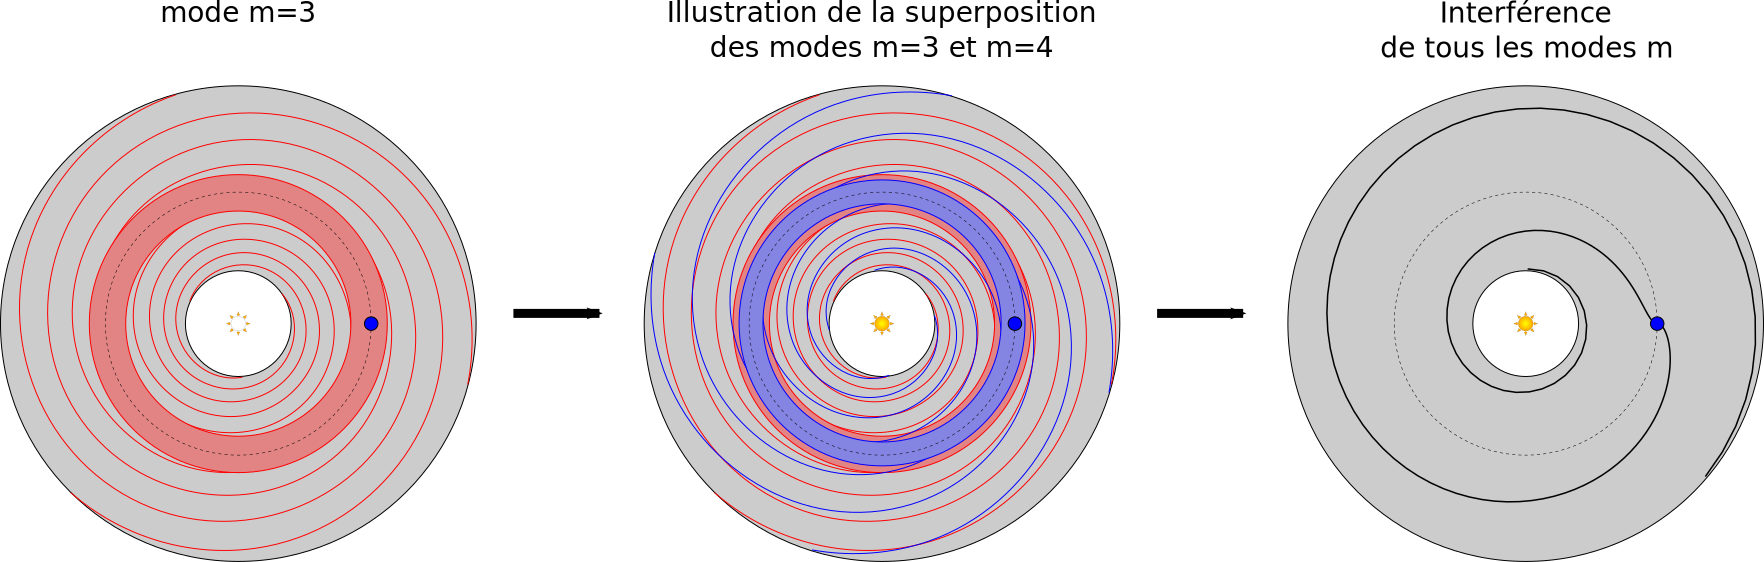
\includegraphics[width=0.49\textwidth]{figure/migration_map/details/lindblad_torque.pdf}}\hfill
\subfloat[Horseshoe Entropy related torque]{\includegraphics[width=0.49\textwidth]{%
figure/migration_map/details/ent_hs_torque.pdf}}

\caption{Evolution des deux couples les plus importants vis à vis de la carte de migration, le couple de Lindblad et la partie non saturée du couple de corotation liée au gradient d'entropie. En effet, ces deux couples sont quantitativement plus grand que tous les autres. Ici, seule la partie non-saturée du couple de corotation est représentée.}\label{fig:details_maps}
\end{figure}

Sur \reffig{fig:details_maps} sont représentés les deux couples les plus importants en terme d'amplitude (tant négative pour le couple de Lindblad $\Gamma_L$, que positive pour la partie du couple de corotation non saturée liée au gradient d'entropie $\Gamma_\text{ent,hs}$. Ici, c'est bien la partie non saturée qui est représentée \og fully unsaturated\fg. On ne tiens pas compte de la diffusion. On constate alors que sans tenir compte de la diffusion, les couples sont totalement indépendants de la masse. 

\begin{figure}[htb]
\centering
\subfloat[$t_\text{rad}/t_\text{U-turn}$]{\label{fig:linear_rad}\includegraphics[width=0.49\textwidth]{figure/timescales/linear_rad.pdf}}\hfill
\subfloat[$(t_\text{lib}/2)/t_\text{visc}$]{\label{fig:sat_visc}\includegraphics[width=0.49\textwidth]{%
figure/timescales/sat_visc.pdf}}

\caption{Comparaison des différents temps caractéristiques influençant le couple de corotation. Ces inéquations sont détaillées dans \refsec{sec:couple-corotation}. Dans le cas présent, le temps de diffusion radiative est toujours plus court que le temps de diffusion visqueuse, $t_\text{rad}<t_\text{visc}$. Ainsi il ne reste plus que les deux inégalités représentées ici.}\label{fig:timescales_maps}
\end{figure}

\reffig{fig:timescales_maps} représente l'effet de la diffusion sur la carte de migration. Seuls deux cartes sont montrées, contrairement aux quatres que nous pourrions attendre, car $t_\text{rad}<t_\text{visc}$. Ainsi, la double inégalité, qui était scindable en 4 sous-inégalités (deux pour chaque temps de diffusion) devient :
\begin{align}
t_\text{U-turn} < t_\text{diff} < \frac{t_\text{lib}}{2}\\
t_\text{U-turn} < t_\text{rad} < t_\text{visc} < \frac{t_\text{lib}}{2}
\end{align}

À partir de \reffig{fig:timescales_maps} on constate deux choses. La première c'est que la zone de couple nul du bas de la carte de migration, est régie par l'inéquation $t_\text{U-turn} < t_\text{rad}$ \reffig{fig:linear_rad}. C'est surtout visible dans la partie $0-4\unit{UA}$, mais cela reste le principal déterminant du reste cette ligne de couple nul. En dessous de cette ligne, c'est uniquement la partie linéaire du couple de corotation qui subsiste. Le temps de diffusion radiatif $t_\text{rad}$ est trop court pour que la zone fer-à-cheval induise une variation des propriétés du disque lors du demi-tour devant la planète. 

La partie supérieure de la carte, quant à elle, est due à la saturation du couple de corotation, illustrée par l'inégalité $(t_\text{lib}/2) > t_\text{visc}$ qui doit être vérifiée pour que le couple ne sature pas \reffig{fig:sat_visc}. C'est particulièrement visible dans la zone $0-4\unit{UA}$. 

Intéressons nous maintenant aux zones qui ferment verticalement les lignes de couple nul. Dans les parties externes, après $15\unit{UA}$, c'est la conjonction des deux processus de diffusion qui \og ferme\fg le profil de couple. Pour les masses faibles, en dessous de $15-20\mearth$, la migration vers l'intérieur est dur au fait que $t_\text{U-turn} > t_\text{rad}$, c'est alors la valeur linéaire du couple de corotation qui prévaut. Pour les masses plus importantes, le couple de corotation sature car $(t_\text{lib}/2) < t_\text{visc}$. 

Avant $1\unit{UA}$, les deux régions de couples positifs sont séparés. C'est une transition d'opacité à $1\unit{UA}$ environ qui en est la cause, et qui change brusquement les couples de migration, quelle que soit leur origine \reffig{fig:details_maps}. Ce brusque changement d'opacité et de température est la raison de la séparation de la zone de couple positif en deux. Ainsi, les raisons valables à $15\unit{UA}$ le sont ici aussi, mais la variation du couple en fonction de la distance est beaucoup plus grande, de sorte que la position de la zone de convergence semble ne pas dépendre de la masse, contrairement aux parties externes de la carte de migration.

\subsection{Différents types de zone de convergence}\label{sec:CZ-types}
En fonction de la distance, nous pouvons définir des masses critiques extrémales au delà desquelles la migration vers l'extérieur est impossible en raison du temps de diffusion qui est soit trop grand (saturation) soit trop petit (couple linéaire) pour qu'un couple de corotation non saturé puisse exister.

Mais l'information la plus importante de ces cartes de migration est certainement l'évolution du couple en fonction de la distance. Nous pouvons dégager deux types particulier de zones de convergence. 

Le premier type de zone de convergence est ce que nous appellerons une zone de convergence indépendante de la masse. C'est une zone qui se trouve plutôt dans les parties interne du disque. Cette ligne de couple nul dépend très peu de la masse de la planète car une transition d'opacité induit de brusques changements de température. Les couples varient ainsi fortement sur une distance très courte. Cette zone de convergence a deux caractéristiques importantes : 
\begin{enumerate}
\item La position de la zone de convergence ne dépend pas ou peu de la masse de planète
\item La variation du couple de migration autour de la zone de convergence est très forte
\end{enumerate}

Nous pouvons appeler le deuxième type \og zone de convergence dépendant de la masse\fg. En effet, dans les parties externes, le couple varie plus doucement en fonction de la distance. L'influence de la masse est donc plus marqué dans la position de la zone de couple nul. Ce type de zone de convergence a deux caractéristiques importantes : 
\begin{enumerate}
\item La position de la zone de convergence dépend de la masse de la planète. 
\item Le couple de migration varie doucement en fonction de la distance à la zone de convergence
\end{enumerate}

\begin{figure}[htb]
\centering
\includegraphics[width=0.75\linewidth]{figure/total_torque_fixed_m.pdf}
\caption{Évolution du couple total exercé par le disque sur une planète de $7.5\mearth$. }\label{fig:total_torque_fixed_m}
\end{figure}

\reffig{fig:total_torque_fixed_m} illustre les deux zones de convergences. La première près de $1\unit{UA}$, siège d'une variation brutale du couple de migration, et la deuxième (dont la position dépend de la masse de la planète) où la variation du couple de migration est continue. 

Dans la suite, nous avons parfois utilisé des zones de convergences artificielles afin de simplifier les effets, et d'étudier plus facilement un phénomène particulier. Nous avons modélisé les zones de convergence indépendantes de la masse par une tangente hyperbolique dont le zéro se situe à la zone de convergence, et où le couple de migration (positif ou négatif) sature très loin de la zone de convergence \refsec{sec:tanh_indep}. 

Les zones de convergence dépendantes de la masse peuvent être approximées par une variation linéaire de la position de la zone de couple nul en fonction de la masse. Le couple de migration varie quant à lui linéairement en fonction de la distance \refsec{sec:mass_dependant}. 


\subsection{Résonances et Accrétions}
%TODO talk about the difference between mass dep and mass indep accretion, in particular the fact that planet of different masses migrate to different position has an influence on the convergent migration. 
% In particular, mass indep with linear migration can be equivalent to mass-indep with steep transition.

\section{Les Résonances de Moyen Mouvement (MMR)}
\subsection{Définition}\index{résonance!de Moyen Mouvement}\index{Mean Motion Resonance|see{résonance}}
Les \gras[resonance@résonance]{résonances de moyen mouvement} sont des configurations orbitales particulières de deux planètes
dans lesquelles il existe un lien entre les périodes orbitales des planètes. Exemple, si deux planètes sont en résonance
\MMR{3}{2}, ça signifie que la planète interne effectuera 3 orbites pendant que la planète externe en effectuera 2.

Ces configurations particulières confèrent une stabilité accrue aux planètes. Plus la résonance est forte et plus il sera difficile pour les planètes d'en sortir.

\bigskip

On met généralement une résonance sous la forme \MMR{(p+q)}{p} où $p$ et $q$ sont des entiers. Cette forme permet de mettre en
évidence un des paramètres qui permet de rendre compte de la force de la résonance. En effet, plus $q$ est petit et plus la
résonance est forte. Ainsi, les résonances d'ordre 1 ($q=1$) sont les plus fortes. On dit que $q$ est l'ordre de la résonance
(plus l'ordre est petit et plus la résonance est forte). De même, $p$ est le degré de la résonance.

\begin{attention}
Mais ce n'est pas le seul paramètre à prendre en compte pour évaluer la force d'une résonance et je suis bien incapable de tous les décrire.
\end{attention}

Pour une résonance \MMR{(p+q)}{p} on définit un certain nombre d'angles $\theta_i$ dits \gras[angle de résonance]{angles de
résonance} de la forme :
\begin{align}
\theta_{i+1} &=(p+q)\lambda_2 -p\lambda_1 - \left[i\varpi_{1} + (q-i)\varpi_2\right]
\end{align}
avec $i$ allant de $0$ à $q$ ; où $\lambda$ sont les longitudes moyennes, $\varpi$ les longitudes du péricentre et les indices
$1$ et $2$ se réfèrent respectivement à la planète interne et externe. Pour une résonance \MMR{(p+q)}{p} on a donc $q+1$ angles
de résonance.

Les angles de résonances mesurent l'angle entre les deux planètes au point de conjonction. Si un seul de ces angles est en libration (oscillation autour d'une valeur moyenne) au lieu de circuler librement de $0$ à $2\pi$ alors on dit que les planètes sont en résonances. Le nombre d'angles en libration permettra aussi d'avoir une idée de la force de la résonance.

\begin{exemple}
Soit une résonance \MMR{7}{2}, les angles de résonances sont :
\begin{align*}
\theta_1 &= 7 \lambda_2 -2\lambda_1 - 5 \varpi_1\\
\theta_2 &= 7 \lambda_2 -2\lambda_1 - \left( 4 \varpi_1 + 1\varpi_2 \right)\\
\theta_3 &= 7 \lambda_2 -2\lambda_1 - \left( 3 \varpi_1 + 2\varpi_2 \right)\\
\theta_4 &= 7 \lambda_2 -2\lambda_1 - \left( 2 \varpi_1 + 3\varpi_2 \right)\\
\theta_5 &= 7 \lambda_2 -2\lambda_1 - \left( 1 \varpi_1 + 4\varpi_2 \right)\\
\theta_6 &= 7 \lambda_2 -2\lambda_1 - 5 \varpi_2
\end{align*}
\end{exemple}

\begin{remarque}
Les \gras[kirkwood@Kirkwood!lacunes de]{lacunes de Kirkwood} font elles aussi intervenir des résonances mais contrairement à ce qu'on pourrait penser, ces résonances avec Jupiter sont des zones déplétées en astéroïdes. 

La résonance imposte une valeur de $a$, mais des échanges sont possibles entre les deux corps en résonance et il est possible que par ce biais l'excentricité puisse augmenter, et ainsi dépléter la lacune de kirkwood en favorisant les collisions entre les objets en résonance et les autres qui sont dans la ceinture.
\end{remarque}


%TODO MMR : lire a thorough analysis of the dunamics involved the reader should consult (Murray & Dermott, 1999)
%TODO cité depuis chapitre 8 resonant perturbations : 
% useful reviews of the subject, particularly in the context of orbital evolution through resonance, have been given by Greenberg (1977), Peale (1986) and Malhotra (1988).
%TODO 
\subsection{Résonances et excentricité}
Cela dépend de l'ordre et du degré de la résonance, mais les perturbations gravitationnelles mutuelles de deux corps en résonance de moyen mouvement engendrent des modifications des éléments orbitaux de ces derniers. 

En particulier, l'excentricité de deux corps en résonance a tendance à varier augmenter au cours du temps \citep[eq. (8.29)]{murray2000solar}. 

Nous n'allons pas détailler ici le fonctionnement précis des résonances. Plusieurs auteurs traitent de ce sujet \citep{greenberg1977orbit, peale1986orbital, malhotra1988phd}. C'est un sujet extrêmement complexe, que je ne maitrise absolument pas dans les détails. De plus, dans le cadre de notre étude de la formation des planètes, nous sommes dans un cas un peu différent. Les résonances entre planète ont lieu dans un système dissipatif, le disque protoplanétaire, qui agit sur les éléments orbitaux, par exemple en amortissant l'excentricité et l'inclinaison des planètes.

Il est difficile de prendre pour exemple les cas N-corps classiques et essayer de les appliquer dans le disque de gaz. Dans notre cas, l'amortissement de $e$ et $I$ par le disque stabilise les résonances, empêchant les résonances normalement instables de se briser. Bien entendu, les résonances se brisent dans nos systèmes en formation, mais dans des cas beaucoup plus extrêmes, notamment quand on a une chaîne de résonance contenant plusieurs corps, tous en résonance. 

\subsection{Stabilité et ordre des résonances}
\reffig{fig:MMR_statistique} montre l'influence du degré de la résonance sur l'excentricité des deux planètes mises en jeu. On
constate tout d'abord que sur 250 simulations effectuées, aucune ne présente des résonances d'ordre $q\neq 1$. Dans le cas de la
migration, où les planètes veulent sortir de la résonance au travers de leur migration différentielle, seules les migration
d'ordre 1 sont assez fortes pour survivre. 


\begin{figure}[htb]
\centering
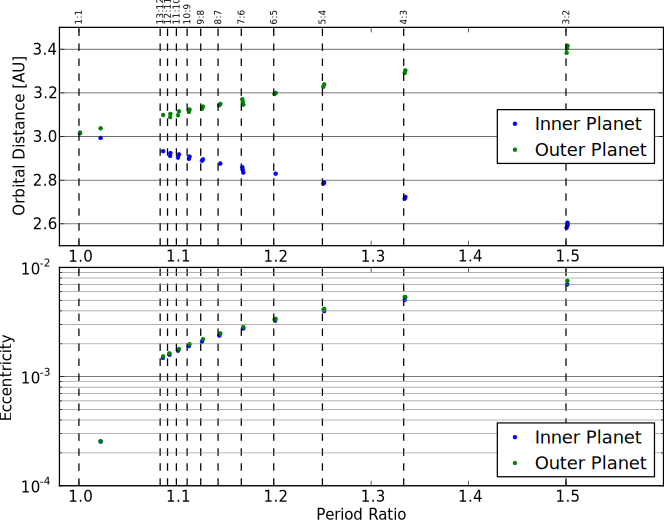
\includegraphics[width=0.75\linewidth]{figure/MMR_statistique.pdf}
\caption{Illustration des différentes résonances possibles et de l'augmentation de l'excentricité qu'elles entrainent. Chaque
simulation contenait deux planètes de $1\mearth$ aléatoirement réparties entre $1$ et $10\unit{AU}$. Chaque point correspond à
une planète. En haut, en fonction du rapport de période, la position finale des planètes est
représentée. En bas, l'excentricité des planètes en fonction du rapport de période avec l'autre planète du système. Une zone de
convergence artificielle à $3\unit{UA}$ a été appliquée. Elle n'a pas d'importance particulier sinon de permettre la formation
de résonances, centrées autour de la même zone du disque, facilitant les études comparatives.}\label{fig:MMR_statistique}
\end{figure}

En fonction du degré de la résonance, l'excentricité des deux corps en résonance diffère. Contrairement à ce qu'on pourrait
penser, ce ne sont pas les résonances de degré élevés qui engendrent les excentricités les plus grandes, même si la distance
entre les deux corps diminue drastiquement. Ainsi, l'excentricité de deux corps sera plus grande s'ils sont en résonance
\MMR{3}{2} par rapport à une \MMR{9}{8}. Ceci vient du fait que même si les planètes sont plus éloignées, dans le cas d'une
résonance \MMR{3}{2}, les conjonctions à l'origine des perturbations gravitationnelles résonances sont beaucoup plus
fréquentes. L'augmentation de l'excentricité est donc beaucoup plus importante \citep{murray2000solar}. 

\subsection{Effet du rapport de masse}
%phd/MMR_mass_ratio
\begin{figure}[htb]
\centering
\includegraphics[width=0.75\linewidth]{figure/MMR_mass_ratio.pdf}
\caption{Résultat de 250 simulations où la première planète, de $10\mearth$ est à $3\unit{UA}$, sur
la zone de convergence artificielle. Une planète externe, placée à $4\unit{UA}$ a une masse
déterminée aléatoirement entre $0.1$ et $10\mearth$. Dans la totalité des simulations, les planètes
se placent en résonance \MMR{3}{2}.}\label{fig:MMR_mass_ratio}
\end{figure}

\reffig{fig:MMR_mass_ratio} se lit de gauche à droite, afin de voir l'effet de l'augmentation de la masse de la planète externe
sur la distance orbitale, l'excentricité et le rapport de périodes orbitales. 

Pour une seconde planète de $0.1\mearth$, on constate que la planète la plus massive se trouve à la position exacte de la
résonance, tandis que la planète externe reste bloquée à $4\unit{UA}$ environ. Les deux planètes ressentent un couple de
migration vers la zone de convergence à $3\unit{UA}$ mais l'inertie de la planète massive est beaucoup plus grande, raison pour
laquelle la planète de $10\mearth$ est à la zone de convergence, la planète de faible masse étant simplement bloquée dans la
résonance. 

On constate de plus qu'en raison de la très grande différence de masse, pour une même résonance l'excentricité des deux
planètes est très différente. La planète la plus massive a une excentricité extrêmement basse, cette dernière étant très peu
sensible aux perturbations de la planète de faible masse. À l'inverse, la planète peu massive est très sensible aux
perturbations de la plus grosse, et son excentricité est bien plus importante, plus de deux ordres de grandeur supérieure.

Pour cette planète externe de $0.1\mearth$ on remarque une dernière chose. Bien qu'en résonance \MMR32, le rapport de période
ne vaut pas exactement $1.5$ comme attendu, mais $1.503$. On retrouve là la divergence du rapport de période pour des
résonances dans un système dissipatifs \citep{batygin2013dissipative}. 

\bigskip

À mesure que l'on augmente la masse de la planète externe, cette dernière pousse petit à petit la planète interne, le rapport
de masse se rapprochant de $1$, elle a peu à peu suffisamment de force pour que l'équilibre des couples de migration se
traduise par une répartition des planètes autour de la zone de convergence. 

Dans le même temps, l'excentricité de la planète interne croit. À mesure que la masse de la planète externe augmente, les
perturbations qu'elle engendre sur l'autre planète augmentent également. Sa masse augmentant, elle devient légèrement moins
sensible aux perturbations de la planète interne et on constate une baisse ténue de l'excentricité de la planète externe. 

Enfin, on remarque que l'écart du rapport de période par rapport à la valeur attendue de $1.5$ pour une résonance \MMR32
augmente avec la masse du deuxième corps. En effet, à mesure que la masse de la planète externe augmente, l'amortissement de
l'excentricité induit par le disque devient plus efficace \citep[eq. (9)]{cresswell2008three}. 

\bigskip

Une fois que le rapport de masse est égal à 1, alors les planètes se placent de part et d'autre de la zone de couple nul, et
les excentricités induites par la résonances deviennent sensiblement égales.

\subsection{Accretion dans une chaîne de résonance}

%TODO